\documentclass[12pt,letterpaper,noanswers]{exam}
\usepackage[usenames,dvipsnames,svgnames,table]{xcolor}
\usepackage[margin=0.9in]{geometry}
\renewcommand{\familydefault}{\sfdefault}
\usepackage{tikz}
\usepackage{multicol}
\pagestyle{head}
\header{AM 111 Class 24}{}{Artificial Neural Networks, p.\thepage}
\runningheadrule
\headrule
\usepackage{siunitx}
\usepackage{graphicx} % more modern
\usepackage{amsmath} 
\usepackage{amssymb} 
\usepackage{hyperref}
\usepackage{tcolorbox}
\usepackage{enumitem}
\def\mbf{\mathbf}
\newcommand{\vc}[1]{\boldsymbol{#1}}
\def\dsst{\displaystyle}
\DeclareMathOperator*{\argmin}{arg\,min} % thin space, limits underneath in displays
\usepackage{listings}
\newcommand{\note}[1]{{#1}} % show notes in red
%\renewcommand{\note}[1]{} % don't display notes

\begin{document}
 \pdfpageheight 11in 
  \pdfpagewidth 8.5in

\noindent 

\section*{Preliminaries}


\begin{itemize}
\itemsep0pt
\item The project log for this week is due on Friday.
\item The final version of your presentation slides are due on Monday Dec 4th.
\item The second quiz is on Thursday.
\end{itemize}


\noindent\textbf{Big picture}

Today: modeling nonlinear functions using artificial neural networks

\vspace{0.2cm}
\hrule
\vspace{0.2cm}

\section*{Artificial neural networks}
\subsection*{Finding the weights: gradient descent}
\note{In our neural network example from the previous class, the weight matrices were taken as given.

In general, weights need to be determined for each layer of the neural net.
\begin{tcolorbox}
Given \textbf{training} data $d_n = \{\vc{x}_n,\hat{\vc{y}}_n\}$ where $n=1,...,N$.  Find weights $\vc{w} = \{W^1,W^2,...,W^L\}$ to minimize the \textbf{error} between the observations, $\hat{\vc{y}}_n$ and the model output.

This is an optimization problem.

%For now we will consider the $2$-norm for the error function.  See \cite{Goodfellow-et-al-2016} \S 6.2.2.2 and \S 6.2.2.3 for a discussion of other choices of error function for particular problem types.
\end{tcolorbox}

With an $L$ layer feedforward neural network, our model is \[\vc{y}(\vc{x}_n,\vc{w}) = \phi_L(W^L\phi_{L-1}(...\phi_2(W^2\phi_1(W^1\vc{x}))...)).\] This is a nonlinear function of $\vc{x}$, parameterized by $\vc{w}$.

The choice of error function should depend on the problem type.  See \cite{Goodfellow-et-al-2016} \S 6.2.2.2 and \S 6.2.2.3 for a discussion of choices of error function for categorical data.  For these notes, we will choose a sum of squares error.  Let \[E_n(\vc{w}) = \dfrac{1}{2}\left(\hat{\vc{y}}_n-\vc{y}(\vc{x}_n,\vc{w})\right)\cdot\left(\hat{\vc{y}}_n-\vc{y}(\vc{x}_n,\vc{w})\right).\]
Let the overall error on the training data set be the sum of the errors on individual input-output pairs.
\[E(\vc{w}) = \sum\limits_{n=1}^N E_n(\vc{w}).\]

The optimization problem is to find the set of weights, $\vc{w}^*$, that minimize $E$.  Nonlinearity of $\vc{y}$, and therefore of $E(\vc{w})$ means that optimization methods for finding a global optimum are unlikely to apply. Instead, use an iterative algorithm to improve the weights at each step $\vc{w}$ with a low error using an iterative, gradient based method.  
}
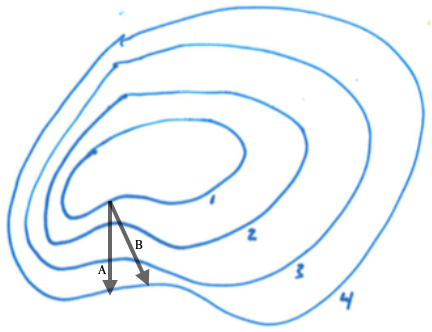
\includegraphics[scale=0.5]{img/C23gradient.png}
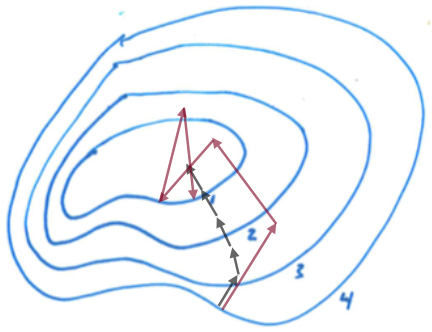
\includegraphics[scale=0.5]{img/C23gradientpath.png}
\begin{enumerate}[resume=classQ]
    \item The contour plots above are showing $E(w_1,w_2)$, a function of two weights.  Each labeled curve is a curve on which the function has a constant value ($E(w_1,w_2) = 3$, for example).
   
   In the plot on the left, one vector is labeled A and the other is labeled B.  Consider the vectors to be originating on the $E = 1$ contour.  Which vector is pointing in a direction closer to the gradient direction?
    \vspace{1cm}
   
\end{enumerate}

\note{\begin{tcolorbox}
This algorithm is sometimes referred to as \textbf{stochastic gradient descent} (but it is not the only algorithm referred to with that terminology).
\begin{itemize}
\itemsep0pt
    \item Let $\vc{w}_1$ be a randomly generated initial set of weights.
    \item Choose one input-output pair from the training data, say $n$, and use the feedforward neural network model to generate $\vc{y}(\vc{x}_n,\vc{w}_1)$ and $E_ n(\vc{w}_1)$.
\item The gradient vector, $\nabla_{\vc{w}}E_n(\vc{w}_1)$ is a vector in the direction of fastest increase of $E_n$ at the point $\vc{w}_1$ (in the weight space). 
\item Update the weights: $\vc{w}_{k+1} = \vc{w}_k - \eta\nabla_{\vc{w}}E_n(\vc{w}_1)$.  $\eta$ is a scaling factor adjust the length of the gradient vector.  It is referred to as the \textbf{learning rate}.
\end{itemize}
\end{tcolorbox}}

\begin{enumerate}[resume=classQ]
 \item In the plot on the right, each vector is drawn to be pointing in the direction of the negative of the gradient (where the gradient is calculated at the tail of the vector).  Which vector path was constructed using a higher learning rate?  How does the error evolve along on each of the paths?
\end{enumerate}

\subsection*{Finding the gradient: back-propagation}

Recall the XOR example from the last class: $y_1 = \phi_2(W^2\phi_1(W^1\vc{x}))$

\newcommand{\inputnum}{3} 
\newcommand{\hiddennum}{3}
\newcommand{\outputnum}{1}
\begin{tikzpicture}
% Input Layer
\foreach \i in {1,...,\inputnum}
{
    \node[circle, 
        minimum size = 6mm,
        fill=orange!30] (Input-\i) at (0,-\i) {};
}
% Hidden Layer
\foreach \i in {1,...,\hiddennum}
{
    \node[circle, 
        minimum size = 6mm,
        fill=teal!50,
        yshift=0*5 mm
    ] (Hidden-\i) at (2.5,-\i) {};
}
% Output Layer
\foreach \i in {1,...,\outputnum}
{
    \node[circle, 
        minimum size = 6mm,
        fill=purple!50,
        yshift=(\outputnum-\inputnum)*5 mm
    ] (Output-\i) at (5,-\i) {};
}
% Connect neurons In-Hidden
\foreach \i in {1,...,\inputnum}
{
    \foreach \j in {2,...,\hiddennum}
    {
        \draw[->, shorten >=15pt] (Input-\i) -- (Hidden-\j);   
    }
}
% Connect neurons Hidden-Out
\foreach \i in {1,...,\hiddennum}
{
    \foreach \j in {1,...,\outputnum}
    {
        \draw[->, shorten >=15pt] (Hidden-\i) -- (Output-\j);
    }
}
% Inputs
\draw (Input-1) node {$1$};
\draw (Input-2) node {$x_1$};
\draw (Input-3) node {$x_2$};
\draw (Hidden-1) node {$1$};
\draw (Hidden-2) node {$z^1_1$};
\draw (Hidden-3) node {$z^1_2$};
\node[left] at (Hidden-2.west) {$a_1^1$};
\node[left] at (Hidden-3.west) {$a_2^1$};
\node[left] at (Output-1.west) {$a_1^2$};
% Outputs
\foreach \i in {1,...,\outputnum}
{            
\draw (Output-\i) node {$y_{\i}$};
    % \draw[->, shorten <=1pt] (Output-\i) -- ++(0.5,0)
    %     node[right]{$y_{\i}$};
}
\end{tikzpicture}

To construct the gradient vector, we want to find $\dfrac{\partial E_n}{\partial w^k_{ji}}$ for each weight $w_{ji}^k$.
\begin{enumerate}[resume=classQ]
\item 
\begin{parts}
\item
Which arrow is associated with $w^1_{21}$?

\emph{Recall that for unit $j$ in the first layer, $a_j^1 = \sum\limits_{i=0}^{2} w_{ji}^1x_i.$}

\item How many weights are there in this XOR example?

\item By the chain rule, $\dfrac{\partial E_n}{\partial w_{ji}^k} = \dfrac{\partial E_n}{\partial a_j^k}\dfrac{\partial a_j^k}{\partial w_{ji}^k}$.  Find $\dfrac{\partial a_2^1}{\partial w_{20}^1}$.  Also find $\dfrac{\partial a_2^1}{\partial w_{21}^1}$.
\vspace{1cm}
\end{parts}
\end{enumerate}
\note{\begin{tcolorbox}
 By the chain rule, $\dfrac{\partial E_n}{\partial w_{ji}^k} = \dfrac{\partial E_n}{\partial a_j^k}\dfrac{\partial a_j^k}{\partial w_{ji}^k} = \dfrac{\partial E_n}{\partial a_j^k}z_i^{k-1}$.
 
 Let $\delta_j^k = \dfrac{\partial E_n}{\partial a_j^k}$, so $\dfrac{\partial E_n}{\partial w_{ji}^k} = \delta_j^k z_i^{k-1}$.
\end{tcolorbox}}
\begin{enumerate}[resume=classQ]
\item Assume you know $\delta_1^2$.
\begin{parts}
\item Which node is associated with $\delta_1^2$?
\item By the chain rule, $\delta_2^1 = \dfrac{\partial E_n}{\partial a_2^1} = \dfrac{\partial E_n}{\partial a_1^2}\dfrac{\partial a_1^2}{\partial a_2^1} = \delta_1^2\dfrac{\partial a_1^2}{\partial a_2^1}$.  We have $a_1^2 = \sum\limits_{i=0}^2 w_{1i}^2z_i^1=\sum\limits_{i=0}^2 w_{1i}^2\varphi_1(a_i^1)$.

Find $\dfrac{\partial a_1^2}{\partial a_2^1}$ and use it to write an expression for $\delta_2^1$ in terms of $\delta_1^2$.
\vspace{1in}

\item Add a second output node, $y_2$, associated with $a_2^2$.  Assume you know $\delta_2^2$.  In this case, $\displaystyle\delta_2^1 = \dfrac{\partial E_n}{\partial a_2^1} = \sum\limits_{m=1}^2 \dfrac{\partial E_n}{\partial a_m^2}\dfrac{\partial a_m^2}{\partial a_2^1}$

Modify your work from (b) to write $\displaystyle\delta_2^1$ as a sum in terms of $\delta_m^2$.
\vspace{1in}

\end{parts}
\end{enumerate}
\note{\begin{tcolorbox}
We can write $\displaystyle\delta_j^k=\dfrac{\partial E_n}{\partial a_j^k}  = \sum\limits_m \dfrac{\partial E_n}{\partial a_m^{k+1}}\dfrac{\partial a_m^{k+1}}{\partial a_j^k}$.  Replacing $\dfrac{\partial a_m^{k+1}}{\partial a_j^k}$ with $\delta_m^{k+1}w^{k+1}_{mj}$, we have

\[\displaystyle\delta_j^k= \sum\limits_m \delta^{k+1}_m \varphi'_k(a_j^k)w^{k+1}_{mj} = \varphi'_k(a_j^k)\sum\limits_m \delta^{k+1}_m w^{k+1}_{mj}.\]

This can be written as a matrix multiplication with the transpose of $W^{k+1}$: \[\delta_j^k = \varphi'_k(a_j^k)(W^{(k+1)T}\vc{\delta}^{k+1})_j\]

Assume that the $a_j^k$ and $z_j^k$ values are saved when constructing $\vc{y}_n$ for a particular input $\vc{x}_n$.  If we have $\vc{\delta}^L$ where $L$ is the final layer, we can construct $\vc{\delta}^{L-1}$ from $\vc{\delta}^L$, $\varphi'(a_j^{L-1})$, and $W^{L}$.  Once we have $\vc{\delta}^{L-1}$ we can construct $\vc{\delta}^{L-2}$, and so on.  This backwards traversal of the network to construct the $\delta_j^k$ gives us the name \textbf{back-propagation}.

Once we have the $\delta_j^k$, the elements of the gradient vector are given by $\dfrac{\partial E_n}{\partial w_{ji}^k} = \delta_j^k z_i^{k-1}$
\end{tcolorbox}}


\subsection*{Example: MNIST}

This example uses the MNIST (modified NIST) handwriting dataset \cite{lecun1998gradient}.

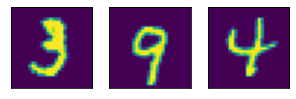
\includegraphics{img/C23mnist.png}

\note{\begin{tcolorbox}
\begin{itemize}
\itemsep0pt
    \item The input is $28\times 28$ ($784$) pixels with values from $0$ to $255$.  The output is a digit, $0,1,...,9$.
\item To set up the model: the input layer has $784$ nodes.  Use one hidden layer with $300$ nodes.  For the output layer, use $10$ nodes, with each encoding one digit, $0$-$9$.  This will represent the digit $3$ by $0,0,0,1,0,0,0,0,0,0$
\item For the activation function, choose the logistic, $\sigma(x)$ for $\varphi_1$ and $\varphi_2$.
\item For the error function: use a sum of squares.  Let $y_0,...,y_9$ be the output of the nodes (corresponding to digits $0$ to $9$) and $\hat{y}_0^n$,...,$\hat{y}_9^n$ be the true values for a training data $n$. 

Let $\vc{e} = \vc{\hat{y}}^n-\vc{y}$, and $E_n(\vc{w}) = \vc{e}\cdot\vc{e} = \sum\limits_{i=0}^9 (\hat{y}_i^n-y_i)^2$
\end{itemize}
\end{tcolorbox}}

\renewcommand{\inputnum}{1} 
\renewcommand{\hiddennum}{1}
\renewcommand{\outputnum}{1}
\begin{tikzpicture}
% Input Layer
\foreach \i in {1,...,\inputnum}
{
    \node[circle, 
        minimum size = 8mm,
        fill=orange!30] (Input-\i) at (0,-\i) {};
}
% Hidden Layer
\foreach \i in {1,...,\hiddennum}
{
    \node[circle, 
        minimum size = 8mm,
        fill=teal!50,
        yshift=0*5 mm
    ] (Hidden-\i) at (2.5,-\i) {};
}
% Output Layer
\foreach \i in {1,...,\outputnum}
{
    \node[circle, 
        minimum size = 8mm,
        fill=purple!50,
        yshift=(\outputnum-\inputnum)*5 mm
    ] (Output-\i) at (5,-\i) {};
}
% Connect neurons In-Hidden
\foreach \i in {1,...,\inputnum}
{
    \foreach \j in {1,...,\hiddennum}
    {
        \draw[->, shorten >=1pt] (Input-\i) -- (Hidden-\j);   
    }
}
% Connect neurons Hidden-Out
\foreach \i in {1,...,\hiddennum}
{
    \foreach \j in {1,...,\outputnum}
    {
        \draw[->, shorten >=1pt] (Hidden-\i) -- (Output-\j);
    }
}
\draw (Input-1) node {$784$};
\draw (Hidden-1) node {$300$};
\draw (Output-1) node {$10$};
\end{tikzpicture}
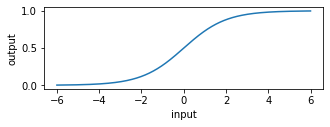
\includegraphics[scale=0.7]{img/C23logistic.png}

\begin{enumerate}[resume=classQ]
\item $\delta_j^2 = \dfrac{\partial E}{\partial a_j^2}$ where $E = \sum\limits_{i=0}^9 (\hat{y}_i^n-y_i)^2 = (\hat{y}_0^n - y_0)^2 + (\hat{y}_1^n - y_1)^2 + ... + (\hat{y}_9^n - y_9)^2$ and $y_i$ is the model output: $y_i = \varphi_2(a_i^2)$.
\begin{parts}
\item $\varphi_2(x) = \sigma(x)$ where $\sigma(x) = (1+e^{-x})^{-1}$.  Find $\dfrac{d\sigma}{dx}$, the derivative of the logistic with respect to $x$.
\vspace{1in}
\item Show that your expression can be rewritten as $\sigma'(x) = \sigma(x)(1-\sigma(x))$
\vspace{1cm}
\item Find $\delta_3^2 = \dfrac{\partial E}{\partial a_3^2} = \dfrac{\partial E}{\partial y_3}\dfrac{\partial y_3}{\partial a_3^2}$.
\vspace{1in}

\item Show that your expression for $\delta_3^2$ can be written as $-2e_{3}y_3(1-y_3)$, where $e_3 = \hat{y}_3^n-y_3$
\vspace{1cm}
\end{parts}

From this, we have $\dfrac{\partial E_n}{\partial w_{ji}^2} = \delta_j^2 z_i^{1} = -2e_{j}y_j(1-y_j)z_i^1$

\end{enumerate}
\note{\begin{tcolorbox}
For this example, $\dfrac{\partial E_n}{\partial w_{ji}^2} = \delta_j^2 z_i^{1} = -2e_{j}y_j(1-y_j)z_i^1$.

What about
$\dfrac{\partial E_n}{\partial w_{ji}^1} = \delta_j^1 x_i = \sigma'(a_j^1)(W^{2T}\vc{\delta}^2)_j x_i$? 

We have $\sigma'(a_j^1) = \sigma(a_j^1)(1-\sigma(a_j^1)) = z_j^1(1-z_j^1)$ so 
$\dfrac{\partial E_n}{\partial w_{ji}^1} =  z_j^1(1-z_j^1)(W^{2T}\vc{\delta}^2)_j x_i$ where $(W^{2T}\vc{\delta}^2)_j = \sum\limits_m w_{mj}^2(-2e_my_m(1-y_m))$.

Let $e_j^1 = \sum\limits_m w_{mj}^2(e_my_m(1-y_m))$.  Then $\dfrac{\partial E_n}{\partial w_{ji}^1} =  -2e^1_jz_j^1(1-z_j^1)x_i$
\end{tcolorbox}}
\subsection*{More MNIST}
The MNIST training and test files are on Canvas and in the \texttt{shared\_data} folder of FAS On Demand.
\begin{enumerate}[resume=classQ]
\item Using C23mnist.ipynb, you might try some of the following:
\begin{parts}
\item Look at the the effect of changing the learning rate.  It is \texttt{alpha} in the code.
\item Test the impact of decreasing the number of runs for training, or of increasing the number.  You might save your weights after every $5000$ updates, and plot your error or your percent correctly classified vs the number of updates used to create the weights.
\item Remove the hidden layer, add a second hidden layer, or adjust the number of units in the hidden layer.
\item Backpropagate the signal, rather than the error, for $[0,0,1,...0]$ (the number $2$) or for a different number to generate a $784$-element vector.  Convert that to an image, and plot it.  What do you see?

\end{parts}
\end{enumerate}

\noindent Below left: the number of connections between neurons in 10 examples of artificial neural networks, plotted vs the year they were published.

\noindent Below right: the size of artificial neural networks for 20 examples, plotted vs the year they were published.

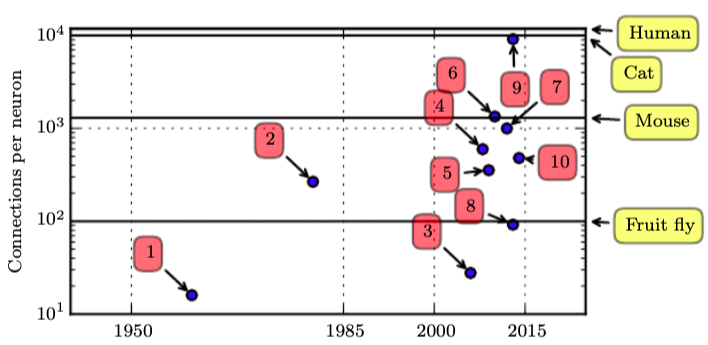
\includegraphics[width=0.45\linewidth]{img/C22neuronconnections.png}
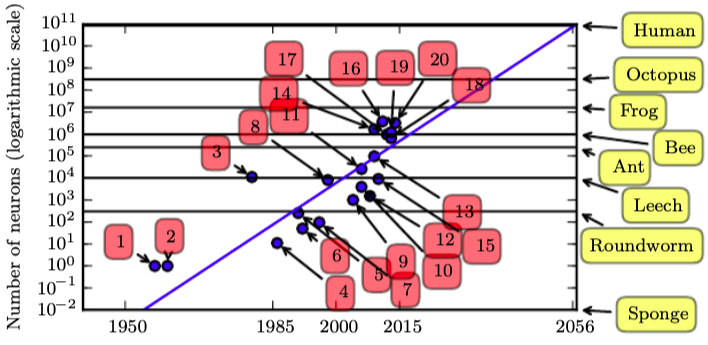
\includegraphics[width=0.45\linewidth]{img/C22neurons.png}
\cite{Goodfellow-et-al-2016}

\bibliographystyle{plain}
\bibliography{AM111references}

\end{document}